\documentclass[twoside,10pt]{article}
\usepackage{amsmath,amsfonts,amsthm,fullpage}
\usepackage{algorithm}
\usepackage{algorithmic}
\usepackage{graphicx}


\begin{document}

\title{ISYE 6740 Fall 2020\\ Homework 1}
%\author{Yao Xie}
\date{}

\maketitle



\section{Clustering [25 points]}



Given $m$ data points $\text x^i$, $i=1,\dots, m$, $K$-means clustering algorithm groups them into $k$ clusters by minimizing the distortion function over $\{ r^{ij}, \mu^j \}$
$$J=\sum_{i=1}^m\sum_{j=1}^k r^{ij} \|\text x^i-\mu^j\|^2,$$
where $r^{ij}=1$ if $\text x^i$ belongs to the $j$-th cluster and $r^{ij}=0$ otherwise.

\begin{enumerate}

\item (5 points) Prove (using mathematical arguments) that using the squared Euclidean distance $\|\text x^i-\mu^j\|^2$ as the dissimilarity function and minimizing the distortion function, we will have 
   $$\mu^j=\frac{\sum_i r^{ij} \text x^i}{\sum_i r^{ij}}.$$
   That is, $\mu^j$ is the center of $j$-th cluster. 
   
   \item (5 points) Discuss qualitatively how the algorithm will change if we replace the similarity function (the squared $\ell_2$ distance here) by a general similar measure $d(x, y)$ (a legitimate measure that satisfies the requirements to be a similarity measure).
   
   
\item (5 points) Prove (using mathematical arguments) that $K$-means algorithm converges to a local optimum in finite steps. 

\item (10 points) Calculate $k$-means by hands.  Given $5$ data points configuration in Figure 1. Assume $k = 2$ and use Manhattan distance (a.k.a. the $\ell_1$ distance: given two 2-dimensional points $(x_1, y_1)$ and $(x_2, y_2)$, their distance is $|x_1 - x_2| + |y_1 - y_2|$).  Assuming the initialization of centroid as shown, after one iteration of k-means algorithm, answer the following questions. 

\begin{enumerate}
\item Show the cluster assignment;
\item Show the location of the new center;
\item Will it terminate in one step?
\end{enumerate}

\begin{figure}[h!]
\begin{center}
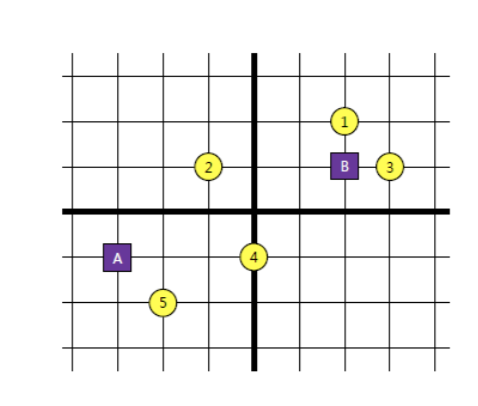
\includegraphics[width = 0.4\textwidth]{points.png}
\end{center}
\caption{K-means.}
\end{figure}

\end{enumerate}


\section{Image compression using clustering [40 points]}

In this programming assignment, you are going to apply clustering algorithms for image compression. Your task is implementing the clustering parts with two algorithms: \emph{$K$-means} and \emph{$K$-medoids}.  {\bf It is required you implementing the algorithms yourself rather than calling from a package.} %Before starting this assignment, we strongly recommend reading PRML Section 9.1.1, page 428 -- 430.

\subsubsection*{$K$-medoids}

In class, we learned that the basic $K$-means works in Euclidean space for computing distance between data points as well as for updating centroids by arithmetic mean. Sometimes, however, the dataset may work better with other distance measures. It is sometimes even impossible to compute arithmetic mean if a feature is categorical, e.g, gender or nationality of a person. With $K$-medoids, you choose a representative data point for each cluster instead of computing their average. Please note that $K$-medoid is different from generalized $K$-means: Generalized $K$-means still computes centre of a cluster is not necessarily one of the input data points (it is a point that minimizes the overall distance to all points in a cluster in a chosen distance metric). 

Given $m$ data points $\text x^i (i = 1, \ldots, m)$, $K$-medoids clustering algorithm groups them into $K$ clusters by minimizing the distortion function $J = \sum_{i=1}^m \sum_{j=1}^k r^{ij} D(\text x^i, \mu^j)$,
where $D(\text x, \text y)$ is a distance measure between two vectors $\text x$ and $\text y$ in same size (in case of $K$-means, $D(x, y) = \| \text x - \text y \|^2$), $\mu^j$ is the center of $j$-th cluster; and $r^{ij} = 1$ if $\text x^n$ belongs to the $k$-th cluster and $r^{ij} = 0$ otherwise. In this exercise, we will use the following iterative procedure:

\begin{itemize}
  \item Initialize the cluster center $\mu^j$, $j = 1, ..., k$.
  \item Iterate until convergence:
  \begin{itemize}
    \item Update the cluster assignments for every data point $\text x^i$: $r^{ij} = 1$ if $j = \arg\min_j D(\text x^i, \mu^j)$, and $r^{ij} = 0$ otherwise.
    \item Update the center for each cluster $j$: choosing another representative if necessary.
  \end{itemize}
\end{itemize}

There can be many options to implement the procedure; for example, you can try many distance measures in addition to Euclidean distance, and also you can be creative for deciding a better representative of each cluster. We will not restrict these choices in this assignment. You are encouraged to try many distance measures as well as way of choosing representatives (e.g., $\ell_1$ norm).

\subsubsection*{Formatting instruction}


\textbf{Input}
\begin{itemize}
  \item \texttt{pixels}: the input image representation. Each row contains one data point (pixel). For image dataset, it contains 3 columns, each column corresponding to Red, Green, and Blue component. Each component has an integer value between 0 and 255.
  \item \texttt{k}: the number of desired clusters. Too high value of $K$ may result in empty cluster error. Then, you need to reduce it.
\end{itemize}

\textbf{Output}
\begin{itemize}
  \item \texttt{class}: cluster assignment of each data point in pixels. The assignment should be 1, 2, 3, etc. For $k = 5$, for example, each cell of class should be either 1, 2, 3, 4, or 5. The output should be a column vector with \texttt{size(pixels, 1)} elements.
  \item \texttt{centroid}: location of $k$ centroids (or representatives) in your result. With images, each centroid corresponds to the representative color of each cluster. The output should be a matrix with $K$ rows and 3 columns. The range of values should be [0, 255], possibly floating point numbers.
\end{itemize}

\subsubsection*{Hand-in}
Both of your code and report will be evaluated. Upload them together as a zip file. In your report, answer to the following questions:
\begin{enumerate}
  \item (10 points) Within the $k$-medoids framework, you have several choices for detailed implementation. Explain how you designed and implemented details of your $K$-medoids algorithm, including (but not limited to) how you chose representatives of each cluster, what distance measures you tried and chose one, or when you stopped iteration.
  \item (10 points) Attach a picture of your own. We recommend size of $320 \times 240$ or smaller. Run your $k$-medoids implementation with the picture you chose, as well as two pictures provided (\textsf{beach.bmp} and \textsf{football.bmp}), with several different $K$. (e.g, small values like 2 or 3, large values like 16 or 32) What did you observe with different $K$? How long does it take to converge for each $K$? Please write in your report. 
  \item (10 points) Run your $k$-medoids implementation with different initial centroids/representatives. Does it affect final result? Do you see same or different result for each trial with different initial assignments? (We usually randomize initial location of centroids in general. To answer this question, an intentional poor assignment may be useful.) Please write in your report. 
  \item (10 points) Repeat question 2 and 3 with $k$-means. Do you see significant difference between $K$-medoids and $k$-means, in terms of output quality, robustness, or running time? Please write in your report. 
\end{enumerate}


\subsubsection*{Note}
\begin{itemize}
  \item You may see some error message about empty clusters when you use too large $k$. Your implementation should treat this exception as well. That is, do not terminate even if you have an empty cluster, but use smaller number of clusters in that case.

  \item We will grade using test pictures which are not provided. We recommend you to test your code with several different pictures so that you can detect some problems that might happen occasionally. 

  \item If we detect copy from any other student's code or from the web, you will not be eligible for any credit for the entire homework, not just for the programming part. Also, directly calling built-in functions or from other package functions is not allowed.
\end{itemize}



\section{Political blogs dataset [35 points] }

We will study a political blogs dataset first compiled for the paper Lada A. Adamic and Natalie Glance, ``The political blogosphere and the 2004 US Election'', in Proceedings of the WWW-2005 Workshop on the Weblogging Ecosystem (2005). The dataset \textsf{nodes.txt} contains a graph with $n = 1490$ vertices (``nodes'') corresponding to political blogs. Each vertex has a 0-1 label (in the 3rd column) corresponding to the political orientation of that blog. We will consider this as the true label and try to reconstruct the true label from the graph using the spectral clustering on the graph. The dataset \textsf{edges.txt} contains edges between the vertices. You may remove isolated nodes (nodes that are not connected any other nodes). 


\begin{enumerate}
\item (5 points)  Assume the number of clusters in the graph is $k$. Explain the meaning of $k$ here intuitively. 

\item (10 points) Use spectral clustering to find the $k = 2$, $k = 3$, and $k = 4$ clusters in the network of political blogs (each node is a blog, and their edges are defined in the file \textsf{edges.txt}). Then report the majority labels in each cluster, when $k = 2, 3, 4$, respectively. For example, if there are $k = 2$ clusters, and their labels are $\{0, 1, 1, 1\}$ and $\{0, 0, 1\}$ then the majority label for the first cluster is 1 and for the second cluster is 0. {\bf It is required you implementing the algorithms yourself rather than calling from a package.} 

\item (5 points) Now compare the majority label with the individual labels in each cluster, and report the {\it mismatch rate} for each cluster, when $k = 2, 3, 4$. For instance, in the example above, the mismatch rate for the first cluster is 1/4 (only the first node differs from the majority) and the the second cluster is 1/3. 

\item (10 points) Now tune your $k$ and find the number of clusters to achieve a reasonably small {\it mismatch rate}. Please explain how you tune $k$ and what is the achieved mismatch rate.  

\item (5 points) Please explain the finding and what can you learn from this data analysis (e.g., node within same community tend to share the same political view, or now? Did you find blogs that share the same political view more tightly connected than otherwise?)

%\item (10 points) You might observe the accuracy is not as good as you expected (given that there is no coding bugs). What do you think might be the reason, due to the discrepancy from ``theory'' and ``application''? Please write in your report. 

\end{enumerate}




\end{document}
